\section{Introduction}\label{sec:introduction}

\subsection{Monte Carlo Estimation, Variance Reduction, and Multilevel Monte Carlo}
Given a random quantity $P$, the standard Monte Carlo estimator of its expectation
$\mathbb{E}[P]$ is simply the average of $N$ independent samples of 
$P$:

\begin{equation*}
    \mathbb{E}[P] \approx \hat{P}_{MC} = \frac{1}{N} \sum_{n=1}^N P^{(n)}
\end{equation*}

Although conceptually simple, the efficiency and feasibility of the Monte Carlo estimator 
depends heavily on the cost of obtaining a single sample. For straightforward 
numerical integration, 
Monte Carlo sampling is inexpensive. To estimate an integral over the unit cube, such as

\begin{equation*}
    \int_{[0,1]^d} f(x)\,dx = \mathbb{E}[f(X)], \quad X\sim\text{Uniform}[0,1]^d,
\end{equation*}

each sample requires only evaluating the function $f$ at a randomly drawn point $X^{(n)}$, 
incurring an $O(1)$ computational cost per sample. 

However, for stochastic systems described by differential equations, the situation becomes 
significantly more costly. Consider the case where $P=f(X_T)$, with $X_t$ governed by 
a stochastic differential equation (SDE):

\begin{equation*}
    dX_t=\mu(X_t)\,dt+\sigma(X_t)\,dW_t,\quad X_0=x_0.
\end{equation*}

Numerically approximating such an SDE typically involves discretising the interval $[0,T]$ into 
small increments $\Delta t$, generating a sequence of approximations 
$\{X_{t_0}, X_{t_1}, \dots, X_{t_N}\}$, with $t_n=n \Delta t$. The 
Euler-Maruyama scheme provides a simple numerical method:

\begin{equation}\label{eq:euler_maruyama}
    X_{t_{n+1}}=X_{t_n}+\mu(X_{t_n})\Delta t+\sigma(X_{t_n})\Delta W_{t_n},\quad n=0,1,\dots,N-1,
\end{equation}

with increments $\Delta W_{t_n} \sim \mathcal{N}(0, \Delta t)$. Generating each sample thus requires
stepping sequentially through a one-dimensional time grid. As the computational cost 
per sample scales linearly with the number of time steps, the cost per sample grows as 
$O(\Delta t^{-1})$.

This computational challenge is even greater for stochastic partial differential equations (SPDEs).
These are partial differential equations also containing random noise, typically used to 
describe systems that are subject to random fluctuations in their evolutions.
In these problems, the unknown variable $u(x,t)$ is a random field evolving over both spatial and 
possibly temporal domains. This is typically done using finite-difference or finite-element methods.
Each Monte Carlo sample therefore corresponds to solving a high-dimensional system of equations repeatedly at 
each time step. Consequently, the computational cost per sample typically scales 
$O(h^{-gamma})$, where $h$ denotes the spatial discretisation scale and $\gamma \ge d$ with $d$ 
the spatial dimension. Achieving accurate numerical solutions demands fine discretisation, 
driving computational cost dramatically upward.


Compounding this issue, the standard Monte Carlo estimator's convergence is inherently slow. The 
variance of the MC estimator is given by 

\begin{equation*}
    \mathbb{V}[\hat{P}_{MC}] = \frac{\mathbb{V}[P]}{N},
\end{equation*}

implying a standard error decreasing only as $O(N^{-1/2})$. Hence, achieving an accuracy in 
$\hat{P}_{MC}$ of $\varepsilon$ requires $O(\varepsilon^{-2})$ samples. Combined with the high
per-sample cost of SPDE simulations, the total computational cost can 
quickly become prohibitive. 

This motivates the use of \textit{variance reduction techniques}, methods specifically designed to 
achieve the same accuracy using fewer and/or cheaper samples. A classical example is the method of 
\textit{control variates}, in which an auxiliary random quantity $C$, with known expectation 
$\mathbb{E}[C]$, is introduced. A modified Monte Carlo estimator is then defined as

\begin{equation}
    \hat{P}_{CV} = \frac{1}{N}\sum_{n=1}^{N}\left[P^{(n)} - \beta(C^{(n)} - \mathbb{E}[C])\right].
\end{equation}

where $\beta$ is a free parameter. The variance of this estimator is

\begin{align*}
    \mathbb{V}[\hat{P}_{CV}] &= \frac{1}{N}\mathbb{V}[P - \beta(C-\mathbb{E}[C])] \\
     &= \frac{1}{N}\left(\mathbb{V}[P] + \beta^2\mathbb{V}[C] - 2\beta\mathrm{Cov}(P,C)\right).
\end{align*}

This expression is quadratic in $\beta$, and we can determine its minimiser $\beta^*$
by differentiating with respect to $\beta$ and setting the result to zero. This yields

\begin{equation*}
    \beta^* = \frac{\mathrm{Cov}(P, C)}{\mathbb{V}[C]}.
\end{equation*}

Therefore, the minimal variance is equal to

\begin{equation*}
    \mathbb{V}[\hat{P}){CV}] = \frac{1}{N} \left(1 - \rho_{P,C}^2\right), 
    \quad \text{where } \rho_{P,C} = \frac{\mathrm{Cov(P,C)}}{\sqrt{\mathbb{V}[P]\mathbb{V}[C]}}
\end{equation*}

is the correlation between $P$ and $C$. The purpose of this derivation is to demonstrate the control variates
mechanism for achieving variance reduction: \textbf{through introducing correlated auxiliary random 
variables with the target variable $P$, we can reduce the overall variance of our estimator $\hat{P}_{CV}$ 
compared to the standard Monte Carlo estimator $\hat{P}_{MC}$}.

How is correlation achieved? Typically by using common underlying random inputs in a 
a given $P^{(n)}$ and $C^{(n)}$ (for example, the 
same Brownian increments in the Euler-Maruyama discretisation in \eqref{eq:euler_maruyama}).
We can describe each pair of samples $P^{(n)}$ and $C^{(n)}$ as being \textit{coupled}.

The Multilevel Monte Carlo (MLMC) method generalises and extends the idea of control variates in a natural and 
powerful way. Rather than a single auxiliary variable, MLMC constructs a hierarchy of increasingly 
accurate (but more costly) estimators $P_0, P_1, \dots, P_L$, each associated with different discretisation 
parameters (mesh sizes or time steps). Instead of directly estimating the closest approximation $P_L$ 
using the standard Monte Carlo estimator, 
MLMC exploits a telescoping sum:

\begin{equation*}
    \mathbb{E}[P_L] = \mathbb{E}[P_0] + \sum_{\ell =1}^L \mathbb{E}[P_\ell - P_{\ell -1}],
\end{equation*}

and estimates this using independent Monte Carlo estimators at each level, giving the MLMC estimator: 

\begin{equation}\label{eq:mlmc_estimator}
    \hat{P}_{MLMC} = \frac{1}{N_0} \sum_{n=1}^{N_0} P_0^{(n)} + 
    \sum_{\ell=1}^L \frac{1}{N_\ell} \sum_{n=1}^{N_\ell} \left(P_\ell^{(n)} - P_{\ell - 1}^{(n)}\right).
\end{equation}

This can be seen as an extension of the control variates estimator, as $L=1$ would retrive for us the 
$\hat{P}_{CV}$ estimator with $\beta = 1$.
As with control variates, by ensuring each pair $P_\ell, P_{\ell - 1}$ uses the same stochastic inputs 
we can achieve strong correlation and thus variance reduction. Small $\ell$ levels 
correspond to cheap, low-accuracy approximations, while large $\ell$ 
levels are more expensive but more accurate. In the context of SDEs and SPDEs, 
lower $\ell$ samples therefore corresponds to samples obtained with larger discrete intervals or mesh sizes, 
and higher $\ell$ to samples with smaller intervals or mesh sizes. 
Figure \ref{fig:coarse_vs_fine_grid} illustrates this concept with a coarse and a fine grid, typical of a 
mesh that can arise in a finite differences scheme.

Summarily then, MLMC aims to reduce the variance of the estimator $\hat{P}_{MLMC}$ by 
taking a blend of coupled samples across varying levels of accuracy. The goal 
is to achieve a target accuracy $\varepsilon$ in an estimate for a cheaper cost 
than the standard Monte Carlo estimator $\hat{P}_{MC}$. 

Several questions follow. First, in the context of SPDEs, 
what cost reductions does the MLMC method provide over the standard Monte 
Carlo method? Secondly, considering Figure \ref{fig:coarse_vs_fine_grid},
we see that the fine grid contains many more random increments than the coarse
grid. If randomness is injected into the grid at each step at each grid point 
in both cases, then how can samples at different levels be coupled? Are there 
coupling schemes more optimal than others?

This leads us to the goal of this dissertation. In this dissertation we 
aim to address the following:

\begin{figure}[htbp]
    \centering
    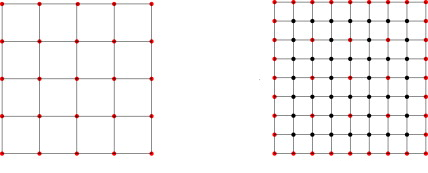
\includegraphics[width=0.6\textwidth]{graphics/fine_grid_vs_coarse_grid.png}
    \caption{An illustrative a coarse and a fine grid}
    \label{fig:coarse_vs_fine_grid}
\end{figure}


\medskip
This dissertation addresses two fundamental questions arising in this context:

\begin{enumerate}
\item What computational savings can be realised by MLMC compared to standard Monte Carlo when solving SPDEs?
\item How should noise be coupled across finite-difference grids of differing resolutions to maximise variance reduction and thereby minimise computational cost?
\end{enumerate}

In answering these questions, we examine various coupling schemes, quantify their effects on MLMC's variance reduction capabilities, and demonstrate how optimal choices lead to substantial computational advantages.
